\chapter{Función de Green.}
%Ref. Herman (2015) - Green's functions and inhomogueneous equations
\section{Introducción.}

La ecuación de onda, la ecuación del calor y la ecuación de Laplace son ecuaciones diferenciales parciales homogéneas típicas. Se pueden escribir en la forma:
\begin{align*}
\mathcal{L} u (x) = 0
\end{align*}
donde $\mathcal{L}$ es un operador diferencial. Por ejemplo, estas ecuaciones se pueden escribir como:
\begin{align*}
\bigg( \pdv[2]{t} - c^{2} \, \laplacian \bigg) \, u &= 0 \\[0.25em]
\bigg( \pdv{t} - k \, \laplacian \bigg) \, u &= 0 \\[0.25em]
\laplacian{u} &= 0
\end{align*}

En este tema revisaremos soluciones de ecuaciones diferenciales parciales no homogéneas, del tipo:
\begin{align*}
\mathcal{L} u (x) = f (x)
\end{align*}
buscando la llamada función de Green. La historia de la función de Green se remonta a 1828, cuando George Green publicó un trabajo en el que buscaba soluciones de la ecuación de Poisson $\laplacian{u} = f$ para el potencial eléctrico $u$ definido dentro de un volumen acotado con condiciones de contorno específicas en la superficie del volumen. Introdujo una función ahora identificada como lo que Riemann más tarde acuñó como la \enquote{función de Green}. En esta parte obtendremos el valor inicial de la función de Green para ecuaciones diferenciales ordinarias. Más adelante en el material de trabajo volveremos a las funciones de Green de condiciones en la frontera y a las funciones de Green para ecuaciones diferenciales parciales.
\par
Como un ejemplo simple, considera la ecuación de Poisson:
\begin{align*}
\laplacian{u} (\vb{r}) = f (\vb{r})
\end{align*}
Sea la ecuación de Poisson dentro de una región $\Omega$ limitada por la superficie $\partial \Omega$ como se muestra en la figura (\ref{fig:figura_07_01}). Esta es la forma no homogénea de la ecuación de Laplace. El término no homogéneo, $f (\vb{r})$, podría representar una fuente de calor en un problema de estado estacionario o una distribución de carga (fuente) en un problema electrostático.
\begin{figure}[H]
    \centering
    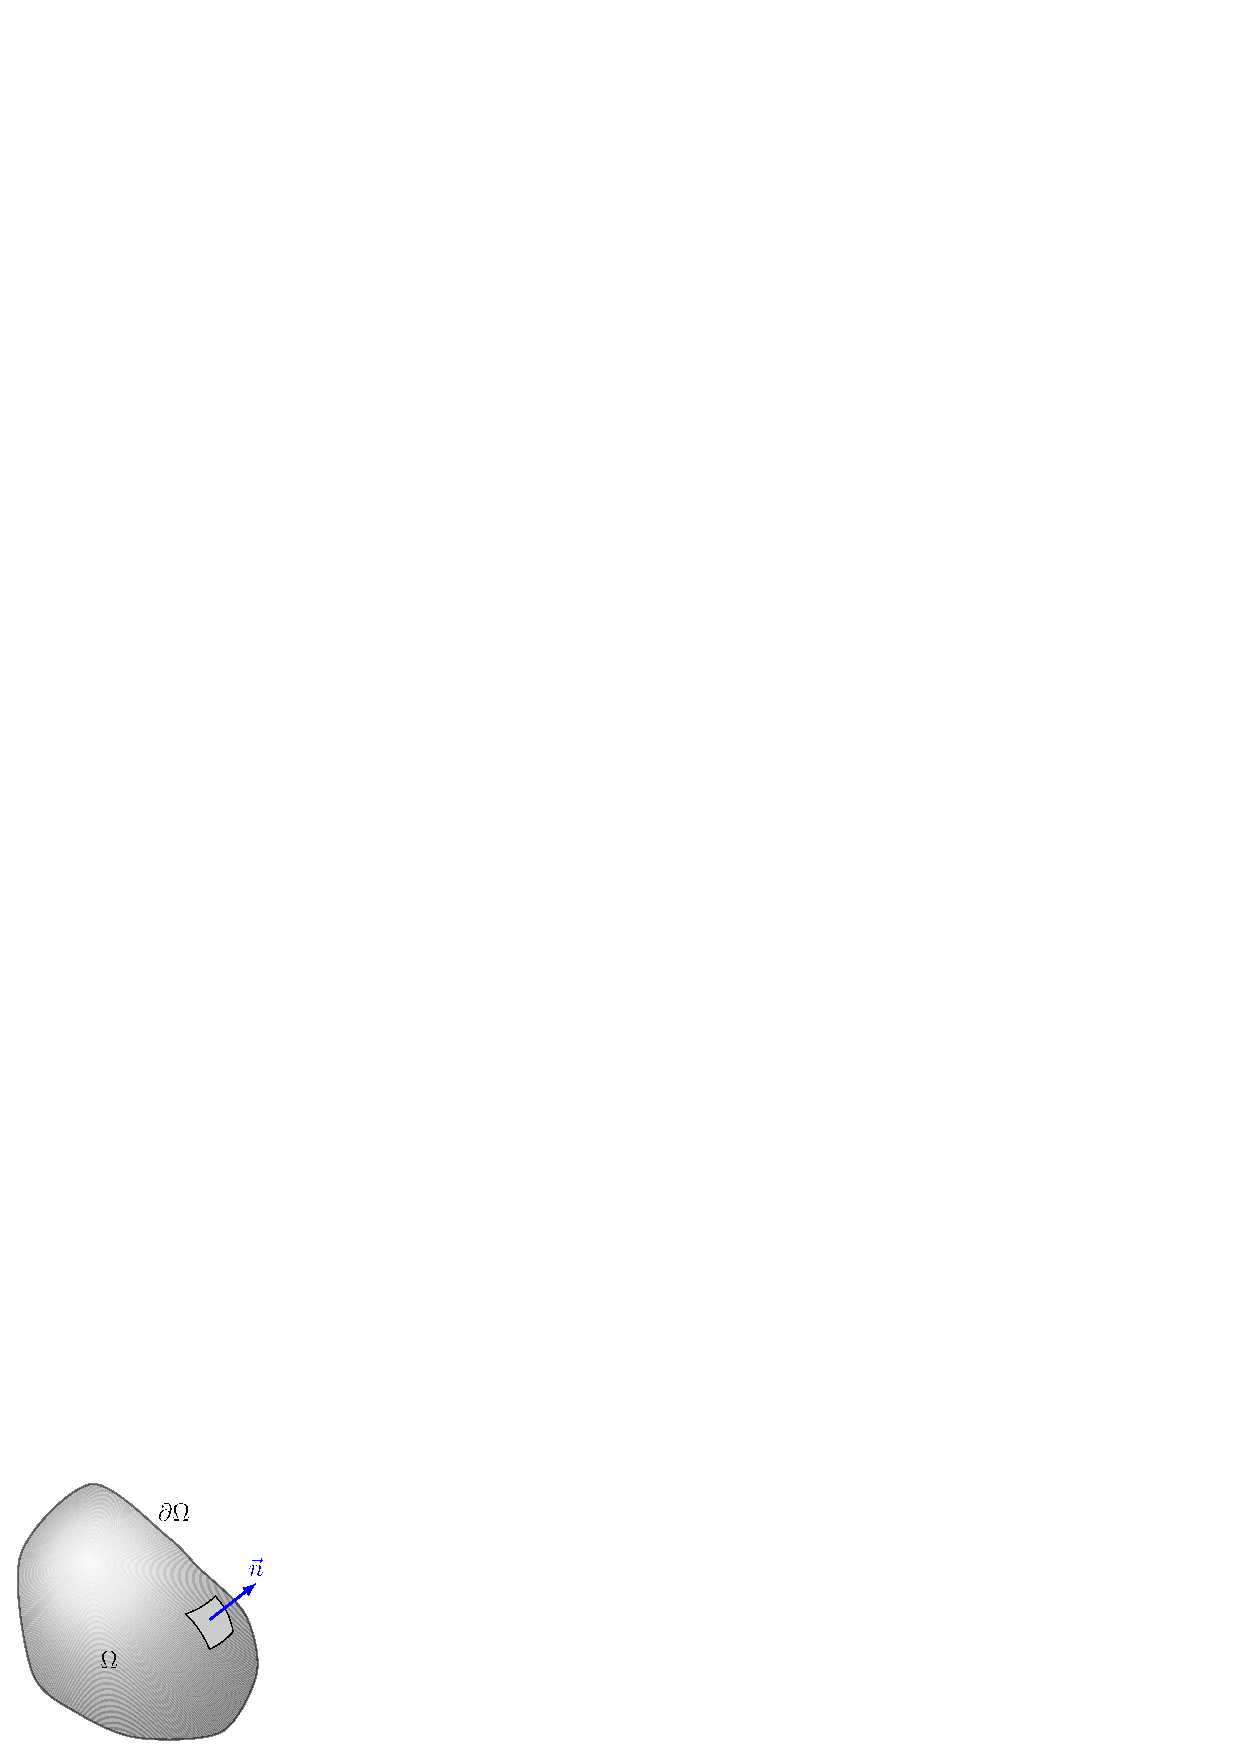
\includegraphics[scale=0.35]{Imagenes/Funcion_Green_01.png}
    \caption{Consideremos la ecuación de Poisson dentro de una región $\Omega$ acotada por una superficie $\partial \Omega$.}
    \label{fig:figura_07_01}
\end{figure}
Ahora pensemos en la fuente como una fuente puntual en la que estamos interesados en la respuesta del sistema a esta fuente puntual. Si la fuente puntual está ubicada en un punto $\vb{\pderivada{r}}$, entonces la respuesta a la fuente puntual podría sentirse en los puntos $\vb{r}$. Llamaremos a esta respuesta $G (\vb{r}, \vb{\pderivada{r}})$. La función de respuesta satisfaría una ecuación de fuente puntual de la forma:
\begin{align*}
\laplacian G (\vb{r}, \vb{\pderivada{r}}) = \delta (\vb{r} - \vb{\pderivada{r}})
\end{align*}
donde $\delta (\vb{r} - \vb{\pderivada{r}})$ es la función delta de Dirac. Una propiedad clave de esta función generalizada\footnote{Revisa el material de trabajo de la función delta de Dirac, en donde encontrarás varias propiedades, entre ellas, la propiedad de filtro.} es la propiedad de filtro:
\begin{align*}
\scaleint{6ex}_{\bs \Omega} \delta (\vb{r} - \vb{\pderivada{r}}) \, f (\vb{r}) \dd{V} = f (\vb{\pderivada{r}})
\end{align*}
La conexión entre la función de Green y la solución a la ecuación de Poisson se encuentra en la segunda identidad de Green:
\begin{align*}
\scaleint{6ex}_{\bs \partial \Omega} \bigg[ \phi \, \grad{\psi} - \psi \, \grad{\phi} \bigg] \cdot \vb{n} \dd{S} = \scaleint{6ex}_{\bs \Omega} \bigg[ \phi \, \laplacian{\psi} - \psi \, \laplacian{\phi} \bigg] \dd{V}
\end{align*}
Haciendo que $\phi = u (\vb{r})$ y $\psi = G (\vb{r}, \vb{\pderivada{r}})$, se tiene que\footnote{Considera que a continuación las integrales de volumen y de superficie, así como la diferenciación usando el operador $\grad$ se realizan usando las $\vb{r}$-coordenadas.}:
\begin{align}
\begin{aligned}[b]
\scaleint{6ex}_{\bs \partial \Omega} \bigg[ u (\vb{r}) \, \grad{G (\vb{r}, \vb{\pderivada{r}})} &- G (\vb{r}, \vb{\pderivada{r}}) \, \grad{u (\vb{r})} \bigg] \cdot \vb{n} \dd{S} = \\[0.5em]
&= \scaleint{6ex}_{\bs \Omega} \bigg[ u (\vb{r}) \, \laplacian{G (\vb{r}, \vb{\pderivada{r}})} - G (\vb{r}, \vb{\pderivada{r}}) \, \laplacian{u (\vb{r})} \bigg] \dd{V} = \\[0.5em]
&= \scaleint{6ex}_{\bs \Omega} \bigg[ u (\vb{r}) \, \delta (\vb{r} - \vb{\pderivada{r}}) - G (\vb{r}, \vb{\pderivada{r}}) \, f (\vb{r}) \bigg] \dd{V} = \\[0.5em]
&= u (\vb{\pderivada{r}}) - \scaleint{6ex}_{\bs \Omega} G (\vb{r}, \vb{\pderivada{r}}) \, f (\vb{r}) \dd{V}
\end{aligned}
\label{eq:ecuacion_07_02}
\end{align}
Al resolver para $u (\vb{\pderivada{r}})$, se tiene que:
\begin{align}
\begin{aligned}[b]
u (\vb{\pderivada{r}}) &= \scaleint{6ex}_{\bs \Omega} G (\vb{r}, \vb{\pderivada{r}}) \, f (\vb{r}) \dd{V} + \\[0.5em]
&+ \scaleint{6ex}_{\bs \partial \Omega} \bigg[ u (\vb{r}) \, \grad{G (\vb{r}, \vb{\pderivada{r}})} - G (\vb{r}, \vb{\pderivada{r}}) \, \grad{u (\vb{r})} \bigg] \cdot \vb{n} \dd{S}
\end{aligned}
\label{eq:ecuacion_07_03}
\end{align}
Si tanto $u (\vb{r})$ como $G (\vb{r}, \vb{\pderivada{r}})$ satisfacen las condiciones de Dirichlet, $u = 0$ en $\partial \Omega$, entonces la última integral se anula y nos queda\footnote{En algunas aplicaciones se presenta la simetría:
\begin{align*}
G (\vb{r}, \vb{\pderivada{r}}) = G (\vb{\pderivada{r}}, \vb{r})
\end{align*}
Por lo que el resultado se puede escribir como:
\begin{align*}
u (\vb{\pderivada{r}}) = \scaleint{6ex}_{\bs \Omega} G (\vb{r}, \vb{\pderivada{r}}) \, f (\vb{\pderivada{r}}) \dd{\pderivada{V}}
\end{align*}
}:
\begin{align*}
u (\vb{\pderivada{r}}) = \scaleint{6ex}_{\bs \Omega} G (\vb{r}, \vb{\pderivada{r}}) \, f (\vb{r}) \dd{V}
\end{align*}
Entonces, si conocemos la función de Green, podemos resolver la ecuación diferencial no homogénea. De hecho, podemos usar la función de Green para resolver problemas de valor límite y valor inicial no homogéneos.

\section{Funciones de Green para valores iniciales.}

En esta parte revisaremos la solución de problemas con valores iniciales que involucran ecuaciones diferenciales no homogéneas utilizando las funciones de Green.
\par
Nuestro objetivo es resolver la ecuación diferencial no homogénea:
\begin{align}
a (t) \, \sderivada{y} (t) + b (t) \, \pderivada{y} (t) + c (t) \, y (t) = f (t)
\label{eq:ecuacion_07_04}
\end{align}
sujeta a las condiciones iniciales:
\begin{align*}
y (0) = y_{0} \hspace{1cm} \pderivada{y} (0) = v_{0}
\end{align*}

Como estamos interesados en problemas de valor inicial, denotaremos la variable independiente como una variable temporal: $t$.
\par
La ec. (\ref{eq:ecuacion_07_04}) se puede escribir de forma compacta como:
\begin{align*}
L [y] = f
\end{align*}
donde $L$ es el operador diferencial:
\begin{align*}
L = a (t) \, \dv[2]{t} + b (t) \, \dv{t} + c (t) 
\end{align*}
Cuya solución está dada por:
\begin{align*}
y = L^{-1} [f]
\end{align*}
El inverso de un operador diferencial es un operador integral, que buscamos escribir en la forma:
\begin{align*}
y (t) = \scaleint{6ex} G (t, \tau) \, f(\tau) \dd{\tau}
\end{align*}
La función $G (t, \tau)$ se conoce como el  \emph{kernel} (núcleo) del operador integral y  se denomina función de Green.
\newpage
Tomando del curso de Ecuaciones Diferenciales I la parte de solución con el \emph{método de variación de parámetros\footnote{Recordemos que este método es un procedimiento útil para la obtención de una solución particular $y_{p} (x)$ de la EDO lineal (no homogénea) y se basa en el conocimiento de la solución general de la lineal homogénea asociada a dicha EDO lineal.}}, hacemos que:
\begin{align}
y_{p} (t) = c_{1} (t) \, y_{1} (t) + c_{2} (t) \, y_{2} (t)
\label{eq:ecuacion_07_05}
\end{align}
encontramos que tenemos que resolver el sistema de ecuaciones:
\begin{align}
\begin{aligned}[b]
\pderivada{c}_{1} (t) \, y_{1} (t) + \pderivada{c}_{2} (t) \, y_{2} (t) &= 0 \\[0.5em]
\pderivada{c}_{1} (t) \, \pderivada{y}_{1} (t) + \pderivada{c}_{2} (t) \, \pderivada{y}_{2} (t) &= \dfrac{f (t)}{q (t)}
\end{aligned}
\label{eq:ecuacion_07_06}
\end{align}
Este sistema se resuelve fácilmente, para obtener entonces:
\begin{align}
\begin{aligned}[b]
\pderivada{c}_{1} (t) &= - \dfrac{f (t) \, y_{2} (t)}{a (t) \big[ y_{1} (t) \, \pderivada{y}_{2} (t)  - \pderivada{y}_{1} (t) \, y_{2} (t) \big]} \\[0.5em]
\pderivada{c}_{2} (t) &= \dfrac{f (t) \, y_{1} (t)}{a (t) \big[ y_{1} (t) \, \pderivada{y}_{2} (t)  - \pderivada{y}_{1} (t) \, y_{2} (t) \big]}
\end{aligned}
\label{eq:ecuacion_07_07}
\end{align}
Notemos que el denominador en estas expresiones involucra el Wronskiano de las soluciones al problema homogéneo, el cual viene dado por el determinante:
\begin{align*}
W (y_{1}, y_{2}) (t) = \mqty|
y_{1} (t) & y_{2} (t) \\
\pderivada{y}_{1} (t) & \pderivada{y}_{2} (t) |
\end{align*}
Cuando $y_{1} (t)$ y $y_{2} (t)$ son linealmente independientes, entonces el Wronskiano no es cero y tenemos garantizada una solución para el sistema anterior.
\par
Entonces, después de una integración, encontramos los parámetros como:
\begin{align}
\begin{aligned}
c_{1} (t) &= - \scaleint{6ex}_{\bs t_{0}}^{t} \dfrac{f (\tau) \, y_{2} (\tau)}{a (\tau) \, W (\tau)} \dd{\tau} \\[0.5em]
c_{2} (t) &= \scaleint{6ex}_{\bs t_{1}}^{t} \dfrac{f (\tau) \, y_{1} (\tau)}{a (\tau) \, W (\tau)} \dd{\tau}
\end{aligned}
\label{eq:ecuacion_07_08}
\end{align}
donde $t_{0}$ y $t_{1}$ son constantes arbitrarias que se determinarán a partir de las condiciones iniciales.
\par
Por lo tanto, la solución particular de la ec. (\ref{eq:ecuacion_07_04}) se puede escribir como:
\begin{align}
y_{p} (t) = y_{2} (t) \scaleint{6ex}_{\bs t_{1}}^{t} \dfrac{f (\tau) \, y_{1} (\tau)}{a (\tau) \, W (\tau)} \dd{\tau} - y_{1} (t) \scaleint{6ex}_{\bs t_{0}}^{t} \dfrac{f (\tau) \, y_{2} (\tau)}{a (\tau) \, W (\tau)} \dd{\tau}
\label{eq:ecuacion_07_09}
\end{align}
Comenzamos con la solución particular de la ec. (\ref{eq:ecuacion_07_09}) de la ED no homogénea (\ref{eq:ecuacion_07_04}). Esto se puede combinar con la solución general del problema homogéneo para dar la solución general de la ecuación diferencial no homogénea:
\begin{align}
y_{p} (t) = c_{1} y_{1} (t) + c_{2} y_{2} (t) +  y_{2} (t) \scaleint{6ex}_{\bs t_{1}}^{t} \dfrac{f (\tau) \, y_{1} (\tau)}{a (\tau) \, W (\tau)} \dd{\tau} - y_{1} (t) \scaleint{6ex}_{\bs t_{0}}^{t} \dfrac{f (\tau) \, y_{2} (\tau)}{a (\tau) \, W (\tau)} \dd{\tau}
\label{eq:ecuacion_07_10}
\end{align}
Sin embargo, se puede encontrar una elección adecuada de $t_{0}$ y $t_{1}$ para que no necesitemos escribir explícitamente la solución al problema homogéneo, $c_{1} y_{1} (t) + c_{2} y_{2} (t)$. No obstante, configurar la solución de esta forma nos permitirá usar $t_{0}$ y $t_{1}$ para determinar soluciones particulares que satisfagan ciertas condiciones homogéneas. En particular, mostraremos que la ec. (\ref{eq:ecuacion_07_10}) se puede escribir en la forma:
\begin{align}
y_{p} (t) = c_{1} y_{1} (t) + c_{2} y_{2} (t) +  y_{2} (t) \scaleint{6ex}_{\bs 0}^{t} G (t,\tau) \, f (\tau) \dd{\tau}
\label{eq:ecuacion_07_11}
\end{align}
donde la función $G (t,\tau)$ será identificada como la función de Green.
\par
El objetivo es entonces desarrollar la técnica de la función de Green para resolver el problema de valor inicial:
\begin{align}
a (t) \, \sderivada{y} (t) + b (t) \, \pderivada{y} (t) + c (t) y(t) = f (t) \hspace{0.6cm} y (0) = y_{0}, \hspace{0.2cm} \pderivada{y} (0) = v_{0}
\label{eq:ecuacion_07_12}
\end{align}
Primero observamos que podemos resolver este problema de valores iniciales resolviendo dos problemas de valor inicial separados. Suponemos que la solución del problema homogéneo satisface las condiciones iniciales originales:
\begin{align}
a (t) \, \sderivada{y}_{h} (t) + b (t) \, \pderivada{y}_{h} (t) + c (t) y_{h} (t) = f (t) \hspace{0.6cm} y_{h} (0) = y_{0}, \hspace{0.2cm} \pderivada{y}_{h} (0) = v_{0}
\label{eq:ecuacion_07_13}
\end{align}
Entonces asumimos que la solución particular satisface el problema:
\begin{align}
a (t) \, \sderivada{y}_{p} (t) + b (t) \, \pderivada{y}_{p} (t) + c (t) y_{h} (t) = f (t) \hspace{0.6cm} y_{p} (0) = y_{0}, \hspace{0.2cm} \pderivada{y}_{p} (0) = v_{0}
\label{eq:ecuacion_07_14}
\end{align}

Dado que la ecuación diferencial es lineal, se sabe que:
\begin{align*}
y (t) = y_{h} (t) + y_{p} (t)
\end{align*}
es una solución a la ecuación no homogénea. También, esta solución satisface las condiciones iniciales:
\begin{align*}
y (0) &= y_{h} (0) + y_{p} (0) = y_{0} + 0 = y_{0} \\[0.5em]
\pderivada{y} (0) &= \pderivada{y}_{h} (0) + \pderivada{y}_{p} (0) = v_{0} + 0 = v_{0}
\end{align*}
Por lo tanto, solo debemos centrarnos en encontrar una solución particular que satisfaga las condiciones iniciales homogéneas. Esto se hará encontrando valores para $t_{0}$ y $t_{1}$ en la ec. (\ref{eq:ecuacion_07_09}) que satisfagan las condiciones iniciales homogéneas: $y_{p} (0) = 0$ y $\pderivada{y}_{p} (0) = 0$
\par
Primero, consideramos $y_{p} (0) = 0$. Tenemos que:
\begin{align}
y_{p} (0) = y_{2} (0) \scaleint{6ex}_{\bs t_{1}}^{0} \dfrac{f (\tau) \, y_{1} (\tau)}{a (\tau) \, W (\tau)} \dd{\tau} - y_{1} (0) \scaleint{6ex}_{\bs t_{0}}^{t} \dfrac{f (\tau) \, y_{2} (\tau)}{a (\tau) \, W (\tau)} \dd{\tau}
\label{eq:ecuacion_07_15}
\end{align}
Aquí, $y_{1} (t)$ y $y_{2} (t)$ se toman como cualquier solución de la ecuación diferencial homogénea. Supongamos que $y_{1} (0) = 0$ y $y_{2} (0) \neq 0$. Entonces, tenemos:
\begin{align}
y_{p} (0) = y_{2} (0) \scaleint{6ex}_{\bs t_{1}}^{0} \dfrac{f (\tau) \, y_{1} (\tau)}{a (\tau) \, W (\tau)} \dd{\tau}
\label{eq:ecuacion_07_16}
\end{align}
Podemos forzar que $y_{p} (0) = 0$ si hacemos que $t_{1} = 0$.
\par
Ahora, consideramos $\pderivada{y}_{p} (0) = 0$. Primero derivamos la solución y encontramos que:
\begin{align}
\pderivada{y}_{p} (t) = \pderivada{y}_{2} (t) \scaleint{6ex}_{\bs 0}^{t} \dfrac{f (\tau) \, y_{1} (\tau)}{a (\tau) \, W (\tau)} \dd{\tau} - \pderivada{y}_{1} (t) \scaleint{6ex}_{\bs t_{0}}^{t} \dfrac{f (\tau) \, y_{2} (\tau)}{a (\tau) \, W (\tau)} \dd{\tau}
\label{eq:ecuacion_07_17}
\end{align}
ya que las contribuciones al diferenciar las integrales se cancelarán. Evaluando este resultado en $t = 0$, tenemos:
\begin{align}
\pderivada{y}_{p} (0) = - \pderivada{y}_{1} (0) \scaleint{6ex}_{\bs t_{0}}^{0} \dfrac{f (\tau) \, y_{2} (\tau)}{a (\tau) \, W (\tau)} \dd{\tau}
\label{eq:ecuacion_07_18}
\end{align}
Suponiendo que $\pderivada{y}_{p} (0) \neq 0$, podemos hacer que $t_{0} = 0$.
\par
Entonces, hemos encontrado que:
\begin{align}
\begin{aligned}[b]
y_{p} (x) &= y_{2} (t) \scaleint{6ex}_{\bs 0}^{t} \dfrac{f (\tau) \, y_{1} (\tau)}{a (\tau) \, W (\tau)} \dd{\tau} - y_{1} (t) \scaleint{6ex}_{\bs t_{0}}^{t} \dfrac{f (\tau) \, y_{2} (\tau)}{a (\tau) \, W (\tau)} \dd{\tau} = \\[0.5em]
&= \scaleint{6ex}_{\bs 0}^{t} \bigg[ \dfrac{y_{1} (\tau) \, y_{2} (t) - y_{1} (t) \, y_{2} (\tau)}{a (\tau) \, W (\tau)} \bigg] \, f (\tau) \dd{\tau}
\end{aligned}
\label{eq:ecuacion_07_19}
\end{align}
Este resultado está en la forma correcta y podemos identificar el valor temporal o inicial: la función de Green. Entonces, la solución particular se da como:
\begin{align}
y_{p} (t) = \scaleint{6ex}_{\bs 0}^{t} G (t, \tau) \, f (\tau) \dd{\tau}
\label{eq:ecuacion_07_20}
\end{align}
donde la condición inicial de la función de Green está definida como:
\begin{align*}
G (t, \tau) = \dfrac{y_{1} (\tau) \, y_{2} (t) - y_{1} (t) \, y_{2} (\tau)}{a (\tau) \, W (\tau)}
\end{align*}

A modo de resumen:
\begin{tcolorbox}[title={\centering Solución para problema de valores iniciales con la función de Green}]

La solución al problema de valores iniciales:
\begin{align*}
a (t) \, \sderivada{y} (t) + b (t) \pderivada{y} (t) + c (t) \, y (t) = f (t) \hspace{0.6cm} y (0) = y_{0}, \hspace{0.2cm} \pderivada{y} (0) = v_{0}
\end{align*}
es de la forma:
\begin{align}
y (t) = y_{h} (t) + \scaleint{6ex}_{\bs 0}^{t} G (t, \tau) \, f (t) \dd{\tau}
\label{eq:ecuacion_07_21}
\end{align}
donde:
\begin{align}
G (t, \tau) = \dfrac{y_{1} (\tau) \, y_{2} (t) - y_{1} (t) \, y_{2} (\tau)}{a (\tau) \, W (\tau)}
\label{eq:ecuacion_07_22}
\end{align}
es la función de Green, $y_{1}$, $y_{2}$, $y_{h}$ son soluciones de la ecuación homogénea que satisfacen:
\begin{align*}
y_{1} (0) = 0, \hspace{0.2cm} y_{2} (0) \neq 0, \hspace{0.2cm} \pderivada{y}_{1} (0) \neq 0, \hspace{0.2cm} \pderivada{y}_{2} (0) = 0, \hspace{0.2cm} y_{h} (0) = y_{0}, \hspace{0.2cm} \pderivada{y}_{h} (0) = v_{0}
\end{align*}
\end{tcolorbox}
\begin{ejemplo}
Resolvamos el problema del oscilador forzado:
\begin{align*}
\sderivada{x} + x = 2 \, \cos t, \hspace{0.5cm} x (0) = 4, \hspace{0.2cm} \pderivada{x} (0) = 0
\end{align*}
Primero resolvemos el problema homogéneo con las condiciones iniciales no homogéneas:
\begin{align*}
\sderivada{x}_{h} + x_{h} = 0, \hspace{0.5cm} x_{h} (0) = 4, \hspace{0.2cm} \pderivada{x}_{h} (0) = 0
\end{align*}
Cuya solución se obtiene fácilmente: $x_{h} (t) = 4 \, \cos t$, que se presenta en la figura (\ref{fig:figura_01}).
\par
A continuación, construimos la función de Green. Necesitamos dos soluciones linealmente independientes, $y_{1} (x)$, $y_{2} (x)$, para la ecuación diferencial homogénea que satisfaga diferentes condiciones homogéneas, $y_{1} (0) = 0$ y $\pderivada{y}_{2} (0) = 0$. Las soluciones más simples son $y_{1} (t) = \sen t$ y $y_{2} (t) = \cos t$.
\par
El Wronskiano para este ejemplo es:
\begin{align*}
W (t) = y_{1} (t) \, \pderivada{y}_{2} (t) - \pderivada{y}_{1} (t) \, y_{2} (t) = - \sin^{2} (t) - \cos^{2} (t) = - 1 
\end{align*}
Dado que en este ejercicio $a (t) = 1$, es posible calcular la función de Green:
\begin{align}
\begin{aligned}[b]
G (t, \tau) &= G (t, \tau) = \dfrac{y_{1} (\tau) \, y_{2} (t) - y_{1} (t) \, y_{2} (\tau)}{a (\tau) \, W (\tau)} = \\[0.5em]
&= \sin t \, \cos \tau - \sin \tau \, \cos t = \\[0.5em]
&= \sin (t - \tau)
\end{aligned}
\label{eq:ecuacion_07_23}
\end{align}
Tomemos en cuenta que la función de Green depende de $t - \tau$. Si bien esto es útil en algunos contextos, usaremos la forma expandida al realizar la integración.
\par
Ahora podemos determinar la solución particular de la ecuación diferencial no homogénea. Tenemos que:
\begin{align}
\begin{aligned}[b]
x_{p} (t) &= \scaleint{6ex}_{\bs 0}^{t} G (t, \tau) \, f (\tau) \dd{\tau} = \\[0.5em]
&= \scaleint{6ex}_{\bs 0}^{t} (\sin t \, \cos \tau - \sin \tau \, \cos t) (2 \, \cos \tau) \dd{\tau} = \\[0.5em]
&= 2 \sin t \, \scaleint{6ex}_{\bs 0}^{t} \cos^{2} \tau \dd{\tau} - 2 \cos t \, \scaleint{6ex}_{\bs 0}^{t} \sin \tau \, \cos \tau \dd{\tau} = \\[0.5em]
&= 2 \sin t \, \bigg[ \dfrac{\tau}{2} + \dfrac{1}{2} \, \sin 2 \tau \bigg] \eval_{0}^{t} - 2 \cos t \, \bigg[ \dfrac{1}{2} \, \sin^{2} \tau \bigg] \eval_{0}^{t} = \\[0.5em]
&= t \, \sin t
\end{aligned}
\label{eq:ecuacion_07_24}
\end{align}

En la figura (\ref{fig:figura_01}) se muestran las soluciones al caso homogéneo como no homogéneo.
\begin{figure}[H]
    \centering
    \includegraphics[scale=0.75]{Imagenes/Plot_Oscilador_Forzado_Green_01.pdf}
    \caption{Soluciones a la EDO en el caso homogéneo y no homogéneo.}
    \label{fig:figura_01}
\end{figure}

Por lo tanto, la solución al problema no homogéneo, es la suma es la solución del problema homogéneo y esta solución particular:
\begin{align*}
x (t) = 4 \, \cos t + t \, \sin t
\end{align*}
La gráfica de la solución se muestra en la figura (\ref{fig:figura_02}):
\begin{figure}[H]
    \centering
    \includegraphics[scale=0.8]{Imagenes/Plot_Oscilador_Forzado_Green_02.pdf}
    \caption{Solución completa a la EDO no homogénea.}
    \label{fig:figura_02}
\end{figure}

\end{ejemplo}

\section{Valores de frontera y funciones de Green.}

En el numeral anterior, resolvimos problemas de valores iniciales no homogéneos usando una función de Green. En esta sección extenderemos este método a la solución de problemas de valores en la frontera no homogéneos usando una función de Green. Recordemos que el objetivo es resolver la ecuación diferencial no homogénea:
\begin{align*}
L [y] = f, \hspace{0.6cm} a \leq x \leq b
\end{align*}
donde $L$ es un operador diferencial y $y (x)$ satisface las condiciones de frontera en $x = a$ y $x = b$. La solución viene dada formalmente por:
\begin{align*}
y = L^{-1} [y]
\end{align*}

El \emph{inverso de un operador diferencial es un operador integral}, que buscamos escribir de la forma:
\begin{align*}
y (x) = \scaleint{6ex}_{a}^{b} G (x, \xi) \, f (\xi) \dd{\xi} 
\end{align*}
La función $G (x, \xi)$ se conoce como el \emph{kernel} (núcleo) del operador integral y se le llama \emph{función de Green}.
\par
Consideraremos problemas de valores en la frontera en forma de Sturm-Liouville\footnote{Este concepto será la parte central del contenido del Tema 3, que sin pérdida de generalidad, podemos mencionar en este momento.}:
\begin{align}
\dv{x} \bigg[ p (x) \, \dv{y (x)}{x} \bigg] + q (x) \, y (x) = f (x), \hspace{0.6cm} a < x < b
\label{eq:ecuacion_07_25}
\end{align}
con valores fijos de $y (x)$ en la frontera, $y (a) = 0$ y $y (b) = 0$. Sin embargo, la teoría general funciona para otras formas de condiciones de frontera homogéneas.
\par
Buscamos la función de Green resolviendo primero la ecuación diferencial no homogénea usando el método de variación de parámetros. Suponemos una solución particular de la forma
\begin{align*}
y_{p} (x) = c_{1} (x) \, y_{1} (x) + c_{2} (x) \, y_{2} (x)
\end{align*}
que se forma a partir de dos soluciones linealmente independientes del problema homogéneo, $y_{i} (x), i = 1, 2$. Habíamos encontrado que las funciones de los coeficientes satisfacen las ecuaciones:
\begin{align}
\begin{aligned}[b]
\pderivada{c}_{1} (t) \, y_{1} (t) + \pderivada{c}_{2} (t) \, y_{2} (t) &= 0 \\[0.5em]
\pderivada{c}_{1} (t) \, \pderivada{y}_{1} (t) + \pderivada{c}_{2} (t) \, \pderivada{y}_{2} (t) &= \dfrac{f (t)}{q (t)}
\end{aligned}
\label{eq:ecuacion_07_26}
\end{align}
resolviendo este sistema, se obtiene:
\begin{align*}
\pderivada{c}_{1} (x) &= - \dfrac{f \, y_{2}}{p \, W (y_{1}, y_{2})} \\[0.5em]
\pderivada{c}_{2} (x) &= \dfrac{f \, y_{1}}{p \, W (y_{1}, y_{2})}
\end{align*}
donde $W (y_{1}, y_{2}) = y_{1} \, \pderivada{y}_{2} - \pderivada{y}_{1} \, y_{2}$ es el Wronskiano. Integrando las expresiones para sustituirlas de regreso en la solución particular, se encuentra que:
\begin{align*}
y (x) = y_{2} (x) \scaleint{6ex}_{\bs x_{1}}^{x_{2}} \dfrac{f (\xi) \, y_{1} (\xi)}{p (\xi) \, W (\xi)} \dd{\xi} - y_{1} (x) \scaleint{6ex}_{\bs x_{0}}^{x} \dfrac{f (\xi) \, y_{2} (\xi)}{p (\xi) \, W (\xi)} \dd{\xi}
\end{align*}
donde $x_{0}$ y $x_{1}$ se determinarán utilizando las condiciones de frontera. En particular, buscaremos $x_{0}$ y $x_{1}$ para que la solución al problema de valores en la frontera pueda escribirse como una integral simple que involucre una función de Green. %Notemos que podemos absorber la solución del problema homogéneo, yh(x), en las integrales con una elección apropiada de límites en las integrales.
\par
Ahora buscamos satisfacer las condiciones $y (a) = 0$ y $y (b) = 0$. Primero usamos soluciones de la ecuación diferencial homogénea que satisfacen $y_{1} (a) = 0$, $y_{2} (b) = 0$ y $y_{1} (b) \neq 0$, $y_{2} (a) \neq 0$. Evaluando $y (x)$ en $x = 0$, tenemos que:
\begin{align}
\begin{aligned}[b]
y (a) &= y_{2} (a) \scaleint{6ex}_{\bs x_{1}}^{a} \dfrac{f (\xi) \, y_{1} (\xi)}{p (\xi) \, W (\xi)} \dd{\xi} - y_{1} (a) \scaleint{6ex}_{\bs x_{0}}^{a} \dfrac{f (\xi) \, y_{2} (\xi)}{p (\xi) \, W (\xi)} \dd{\xi} = \\[0.5em]
&= y_{2} (a) \scaleint{6ex}_{\bs x_{1}}^{a} \dfrac{f (\xi) \, y_{1} (\xi)}{p (\xi) \, W (\xi)} \dd{\xi}
\end{aligned}
\label{eq:ecuacion_07_27}
\end{align}
Podemos satisfacer la condición en $x = a$ si escogemos $x_{1} = a$. De manera similar, en $x = b$, encontramos que:
\begin{align}
\begin{aligned}[b]
y (b) &= y_{2} (b) \scaleint{6ex}_{\bs x_{1}}^{b} \dfrac{f (\xi) \, y_{1} (\xi)}{p (\xi) \, W (\xi)} \dd{\xi} - y_{1} (b) \scaleint{6ex}_{\bs x_{0}}^{b} \dfrac{f (\xi) \, y_{2} (\xi)}{p (\xi) \, W (\xi)} \dd{\xi} = \\[0.5em]
&= - y_{1} (b) \scaleint{6ex}_{\bs x_{0}}^{b} \dfrac{f (\xi) \, y_{2} (\xi)}{p (\xi) \, W (\xi)} \dd{\xi}
\end{aligned}
\label{eq:ecuacion_07_28}
\end{align}
Esta expresión se anula para $x_{0} = b$.

Así, hemos encontrado que la solución es de la forma:
\begin{align}
y (x) &= y_{2} (x) \scaleint{6ex}_{\bs a}^{x} \dfrac{f (\xi) \, y_{1} (\xi)}{p (\xi) \, W (\xi)} \dd{\xi} - y_{1} (x) \scaleint{6ex}_{\bs b}^{x} \dfrac{f (\xi) \, y_{2} (\xi)}{p (\xi) \, W (\xi)} \dd{\xi}
\label{eq:ecuacion_07_29}
\end{align}
Esta solución se puede escribir en forma compacta tal como lo hicimos para el problema de valores iniciales del numeral anterior. Buscamos una función de Green para que la solución se pueda escribir como una sola integral. Podemos mover las funciones de $x$ debajo de la integral. Además, dado que $a < x < b$, podemos invertir los límites en la segunda integral. Esto nos da:
\begin{align}
y (x) &= \scaleint{6ex}_{\bs x}^{a} \dfrac{f (\xi) \, y_{1} (\xi) \, y_{2} (x)}{p (\xi) \, W (\xi)} \dd{\xi} + \scaleint{6ex}_{\bs x}^{b} \dfrac{f (\xi) \, y_{1} (x) \, y_{2} (\xi)}{p (\xi) \, W (\xi)} \dd{\xi}
\label{eq:ecuacion_07_30}
\end{align}
Este resultado se puede ahora escribir de una manera compacta:
\begin{tcolorbox}[title={\centering Solución para problema de CDF con la función de Green}]

La solución para el problema de condiciones de frontera:
\begin{align}
\begin{aligned}
\dv{x} \bigg[ p (x) \, \dv{y (x)}{x} \bigg] &+ q (x) \, y (x) = f (x), \hspace{0.6cm} a < x < b \\[0.5em]
&y (a) = 0, \hspace{0.4cm} y (b) = 0
\end{aligned}
\label{eq:ecuacion_07_31}
\end{align}
toma la forma:
\begin{align}
y (x) = \scaleint{6ex}_{\bs a}^{b} G (x, \xi) \, f (\xi) \dd{\xi}
\label{eq:ecuacion_07_32}
\end{align}
donde la función de Green es una función en partes definida como:
\begin{align}
G (x, \xi) = \begin{cases}
\dfrac{y_{1} (\xi) \, y_{2} (x)}{p \, W}, & a \leq \xi \leq x \\[0.5em]
\dfrac{y_{1} (x) \, y_{2} (\xi)}{p \, W}, & x \leq \xi \leq b
\end{cases}
\label{eq:ecuacion_07_33}
\end{align}
donde $y_{1} (x)$ y $y_{2} (x)$ son soluciones al problema homogéneo que satisfacen $y_{1} (a) = 0$, $y_{2} (b) = 0$ y $y_{1} (b) \neq 0$, $y_{2} (a) \neq 0$.
\end{tcolorbox}

La función de Green satisface varias propiedades, que revisaremos más adelante. Por ejemplo, la función de Green satisface las condiciones de frontera en $x = a$ y $x = b$. Por lo tanto:
\begin{align*}
G (a, \xi) &= \dfrac{y_{1} (a) \, y_{2} (x)}{p \, W} = 0 \\[0.5em]        
G (b, \xi) &= \dfrac{y_{1} (\xi) \, y_{2} (b)}{p \, W} = 0
\end{align*}
Además, la función de Green es simétrica en sus argumentos. Intercambiando los argumentos nos devuelve:
\begin{align}
G (\xi, x) = \begin{cases}
\dfrac{y_{1} (x) \, y_{2} (\xi)}{p \, W}, & a \leq x \leq \xi \\[0.5em]
\dfrac{y_{1} (\xi) \, y_{2} (x)}{p \, W}, & \xi \leq x \leq b
\end{cases}
\label{eq:ecuacion_07_34}
\end{align}    
Pero revisando de manera cuidadosa a la forma original, tenemos que:
\begin{align*}
G (x, \xi) = G (\xi, x)
\end{align*}

Haremos uso de estas propiedades más adelante para determinar rápidamente las funciones de Green para otros problemas de valores en la frontera.

\begin{ejemplo}
Usando la función de Green para CDF, resuelve el problema:
\begin{align*}
\sderivada{y} = x^{2}, \hspace{0.6cm} y (0) = 0 = y (1)
\end{align*}
Primero resolvemos la ecuación homogénea, $\sderivada{y} = 0$. Después de dos integraciones, tenemos que:
\begin{align*}
y (x) = A \, x + B
\end{align*}
donde falta determinar las constantes $A$ y $B$.
\par
Necesitamos una solución que satisfaga $y_{1} (0) = 0$. Por lo tanto:
\begin{align*}
0 = y_{1} (0) = B
\end{align*}

\end{ejemplo}
Entonces, podemos elegir $y_{1} (x) = x$, ya que $A$ es arbitrario.
\par
La otra solución tiene que satisfacer $y_{2} (1) = 0$. Entonces:
\begin{align*}
0 = y_{2} (1) = A + B
\end{align*}
Esto se puede resolver para $B = - A$. Nuevamente, $A$ es arbitraria y elegimos $A = - 1$. Por tanto:
\begin{align*}
y_{2} (x) = 1 - x
\end{align*}
Las soluciones al problema homogéneo se presentan en la figura (\ref{fig:figura_03}).
\begin{figure}[H]
    \centering
    \includegraphics[scale=0.75]{Imagenes/Plot_EDONH_Green_01.pdf}
    \caption{Soluciones $y_{1} (x)$ y $y_{2} (x)$ para el caso de la ED homogénea.}
    \label{fig:figura_03}
\end{figure}

Para este problema $p (x) = 1$. Así, para $y_{1} (x) = x$ y $y_{2} (x) = 1 - x$, el producto:
\begin{align*}
p (x) \, W (x) =  y_{1} (x) \, \pderivada{y}_{2} (x) - \pderivada{y}_{1} (x) \, y_{2} (x) = x (-1) -  1(1 - x) = - 1
\end{align*}
Tomemos en cuenta que $p (x) \, W (x)$ es una constante, como debería ser.
\par
Ahora construimos la función de Green. Así tenemos:
\begin{align}
G (x, \xi) = \begin{cases}
- \xi \, (1 - x), & 0 \leq \xi \leq x \\
- x \, (1 - \xi), & x \leq \xi \leq 1
\end{cases}
\label{eq:ecuacion_07_35}
\end{align}

Observemos la simetría entre las dos partes de la función de Green. \break \hfill Además, la función de Green satisface condiciones de frontera homogéneas: 
\begin{align*}
G (0, \xi) &= 0, \mbox{ de la parte inferior}, \\[0.5em]
G (1, \xi) &= 0, \mbox{ de la parte superior}
\end{align*}
Finalmente, sustituimos la función de Green en la forma integral de la solución y evaluamos la integral:
\begin{align}
\begin{aligned}[b]
y (x) &= \scaleint{6ex}_{0}^{1} G (x, \xi) \, f (\xi) \dd{\xi} = \\[0.5em]
&= \scaleint{6ex}_{0}^{1} G (x, \xi) \, \xi^{2} \dd{\xi} = \\[0.5em]
&= - \scaleint{6ex}_{0}^{x} \xi \, (1 - x) \, \xi^{2} \dd{\xi} - \scaleint{6ex}_{x}^{1} x \, (1 - \xi) \, \xi^{2} \dd{\xi} = \\[0.5em]
&= - (1 - x) \scaleint{6ex}_{0}^{x} \xi^{3} \dd{\xi} - x \, \scaleint{6ex}_{x}^{1} (\xi^{2} - \xi^{3}) \dd{\xi} = \\[0.5em]
&= - (1 - x) \bigg[ \dfrac{\xi^{4}}{4} \bigg] \eval_{0}^{4} - x \bigg[ \dfrac{\xi^{3}}{3} - \dfrac{\xi^{4}}{4} \bigg] \eval_{x}^{1} = \\[0.5em]
&= \dfrac{1}{4} (1 - x) x^{4} - \dfrac{1}{12} \, x (4 - 3) + \dfrac{1}{12} \, x (4 x^{3} - 3 x^{4}) = \\[0.5em]
&= \dfrac{1}{12} (x^{4} - x)
\end{aligned}
\label{eq:ecuacion_07_36}
\end{align}
Revisando la solución, se verifica fácilmente que la EDO
\begin{align*}
\sderivada{y} = x^{2}
\end{align*}
se satisface para las CDF $y (0) = 0$ y $y (1) = 0$. La solución completa al caso no homogéneo se presenta en la figura (\ref{fig:figura_04}).
\begin{figure}[H]
    \centering
    \includegraphics[scale=0.75]{Imagenes/Plot_EDONH_Green_02.pdf}
    \caption{Solución a la ED no homogénea que cumple con las CDF indicadas en el ejercicio.}
    \label{fig:figura_04}
\end{figure}

\section{Propiedades de la función de Green.}

Hemos mencionado algunas propiedades de las funciones de Green en el último numeral.
\par
En esta parte revisaremos algunas de estas propiedades como una herramienta para construir rápidamente funciones de Green para problemas de valores en la frontera. Enumeramos cinco propiedades básicas:
\begin{enumerate}
\item \textbf{Ecuación diferencial: } La función de Green con valor de frontera satisface la ecuación diferencial:
\begin{align*}
\pdv{x} \bigg[ p (x) \, \pdv{G (x, \xi)}{x} \bigg] + q (x) \, G (x, \xi) = 0, \hspace{0.5cm} x \neq \xi
\end{align*}
Esto se establece fácilmente. Para $x < \xi$ estamos en el  segundo caso y $G (x, \xi)$ es proporcional a $y_{1} (x)$. Así, dado que $y_{1} (x)$ es una solución de la ecuación homogénea, también lo es $G (x, \xi)$. Para $x > \xi$ estamos en el primer caso y $G (x, \xi)$ es proporcional a $y_{2} (x)$. Entonces, una vez más $G (x, \xi)$ es una solución del problema homogéneo.
\item \textbf{Condiciones de frontera :} En el ejemplo del numeral anterior, se vio que $G (a, \xi) = 0$ y $G (b, \xi) = 0$. Por ejemplo, para $x = a$ estamos en el segundo caso y $G (x, \xi)$ es proporcional a $y_{1} (x)$. Por lo tanto, cualquier condición que satisfaga $y_{1} (x)$, $G (x, \xi)$ la satisfará. Se puede hacer una afirmación similar para $x = b$.
\item \textbf{Simetría o reciprocidad :} $G (x, \xi) = G (\xi, x)$.
\par
\noindent
Se demostró esta propiedad en el numeral anterior.
\item \textbf{Continuidad de $\mathbf{G}$ en $x = \xi$ :} $G (\xi^{+}, \xi) = G (\xi^{-}, \xi)$
\par
\noindent
Aquí definimos $\xi^{\pm}$ a través de los límites de una función cuando $x$ tiende a $\xi$ desde arriba o desde abajo En particular:
\begin{align*}
G (\xi^{+}, x) &= \lim_{x \uparrow \xi}, \hspace{0.4cm} x > \xi \\[0.5em]
G (\xi^{-}, x) &= \lim_{x \downarrow \xi}, \hspace{0.4cm} x < \xi
\end{align*}
Haciendo $x = \xi$ en ambos casos, tenemos que:
\begin{align*}
\dfrac{y_{1} (\xi) \, y_{2} (\xi)}{p \, W} = \dfrac{y_{1} (\xi) \, y_{2} (\xi)}{p \, W}
\end{align*}
Por tanto, hemos establecido la continuidad de $G (x, \xi)$ entre los dos casos en $x = \xi$.
\item \textbf{Salto de discontinuidad de $\displaystyle \pdv{G}{x}$ en $x = \xi$ :}
\begin{align*}
\pdv{G (\xi^{+}, \xi)}{x} - \pdv{G (\xi^{-}, \xi)}{x} = \dfrac{1}{p (\xi)}
\end{align*}
Esta propiedad no es tan obvia. Primero calculamos las derivadas observando qué caso está involucrado y luego evaluamos las derivadas y las restamos. Así, tenemos lo siguiente:
\begin{align}
\begin{aligned}[b]
\pdv{G (\xi^{+}, \xi)}{x} - \pdv{G (\xi^{-}, \xi)}{x} &= - \dfrac{1}{p \, W} \, y_{1} (\xi) \, \pderivada{y}_{2} (\xi) + \dfrac{1}{p \, W} \, \pderivada{y}_{1} (\xi) \, y_{2} (\xi) = \\[0.5em]
&= - \dfrac{\pderivada{y}_{1} (\xi) \, y_{2} (\xi) - y_{1} (\xi) \, \pderivada{y}_{2} (\xi)}{p (\xi) \, \big[ y_{1} (\xi) \, \pderivada{y}_{2} (\xi) - \pderivada{y}_{1} (\xi) \, y_{2} (\xi) \big]} = \\[0.5em]
&= \dfrac{1}{p (\xi)}
\end{aligned}
\label{eq:ecuacion_07_37}
\end{align}
\end{enumerate}
Se presenta un resumen de las propiedades de la función de Green con condiciones de frontera basado en la solución anterior.
\begin{tcolorbox}[title={\centering Propiedades de la función de Green}]

\begin{enumerate}
\item \textbf{Ecuación diferencial:}
\begin{align*}
\pdv{x} \bigg[ p (x) \, \pdv{G (x, \xi)}{x} \bigg] + q (x) \, G (x, \xi) = 0, \hspace{0.5cm} x \neq \xi
\end{align*}
\item \textbf{Condiciones de frontera :} Con cualesquiera condiciones $y_{1} (x)$ y $y_{2} (x)$ que se satisfagan, $G (x, \xi)$ se satisface.
\item \textbf{Simetría o reciprocidad :} $G (x, \xi) = G (\xi, x)$
\item \textbf{Continuidad de $\mathbf{G}$ en $x = \xi$ :} $G (\xi^{+}, \xi) = G (\xi^{-}, \xi)$
\item \textbf{Salto de discontinuidad de $\displaystyle \pdv{G}{x}$ en $x = \xi$ :}
\begin{align*}
\pdv{G (\xi^{+}, \xi)}{x} - \pdv{G (\xi^{-}, \xi)}{x} = \dfrac{1}{p (\xi)}
\end{align*}
\end{enumerate}
\end{tcolorbox}
Ahora mostramos cómo el conocimiento y manejo de estas propiedades, permite construir rápidamente una función de Green con un ejemplo.
\begin{ejemplo}
Construye la función de Green para el siguiente problema:
\begin{align*}
\sderivada{y} &+ \omega^{2} \, y = f(x) \hspace{0.6cm} 0 < x < 1 \\[0.5em]
&=y (0) = 0 = y (1) \hspace{0.6cm} \omega \neq 0
\end{align*}
\begin{enumerate}
\item \textbf{Encontrar las soluciones a la ecuación homogénea.}
\par
\noindent
Una solución general a la ecuación homogénea está dada por:
\begin{align*}
y_{h} (x) = c_{1} \, \sin \omega x + c_{2} \, \cos \omega x
\end{align*}
Por lo que, para $x \neq \xi$:
\begin{align*}
G (x, \xi) = c_{1} (\xi) \, \sin \omega x + c_{2} (\xi) \, \cos \omega x
\end{align*}
\item \textbf{Condiciones de frontera.}
\par
\noindent
Primero, tenemos que $G (0, \xi) = 0$ para $0 \leq x \leq \xi$. Así:
\begin{align*}
G (0, \xi) = c_{2} (\xi) \, \cos \omega x = 0
\end{align*}
Entonces:
\begin{align*}
G (x, \xi) = c_{1} (\xi) \, \sin \omega x = 0, \hspace{0.5cm} 0 \leq x \leq \xi
\end{align*}
Segundo, tenemos que $G (1, \xi) = 0$, para $\xi \leq x \leq 1$. Por lo tanto:
\begin{align*}
G (1, \xi) = c_{1} (\xi) \, \sin \omega + c_{2} (\xi) \, \cos \omega = 0
\end{align*}
Se puede elegir una solución haciendo que:
\begin{align*}
c_{2} (\xi) = - c_{1} (\xi) \, \tan \omega
\end{align*}
Esto nos proporciona:
\begin{align*}
G (x, \xi) = c_{1} (\xi) \, \sin \omega x - c_{1} (\xi) \, \tan \omega \, \cos \omega x
\end{align*}
Esto se puede simplificar factorizando el $c_{1} (\xi)$ y colocando los términos restantes sobre un denominador común. El resultado es:
\begin{align}
\begin{aligned}[b]
G (x, \xi) &= \dfrac{c_{1} (\xi)}{\cos \omega} \big[ \sin \omega x \, \cos \omega - \sin \omega \, \cos \omega x \big] = \\[0.5em]
&= - \dfrac{c_{1} (\xi)}{\cos \omega} \, \sin \omega (1 - x)
\end{aligned}
\label{eq:ecuaction_07_38}
\end{align}
Dado que el coeficiente es arbitrario en este punto, podemos escribir el resultado como:
\begin{align*}
G (x, \xi) = d_{1} (\xi) \, \sin \omega (1 - x), \hspace{0.5cm} \xi \leq x \leq 1
\end{align*}
Observamos que podríamos haber comenzado con $y_{2} (x) = \sin \omega (1 - x)$ como una de las soluciones linealmente independientes del problema homogéneo, anticipando que $y_{2} (x)$ satisface la segunda condición de frontera.
\item \textbf{Simetría o reciprocidad.}
\par
\noindent
Si imponemos que $G (x, \xi) = G (\xi, x)$. En este punto tenemos que:
\begin{align*}
G (x, \xi) = \begin{cases}
c_{1} (\xi) \, \sin \omega x & 0 \leq x \leq \xi \\[0.5em]
d_{1} (\xi) \, \sin \omega (1 - x) & \xi \leq x \leq 1
\end{cases}
\end{align*}
Podemos hacer que los casos sean simétricos eligiendo las formas correctas para $c_{1} (\xi)$ y $d_{1} (\xi)$. Elegimos :
\begin{align*}
c_{1} (\xi) &= C \, \sin \omega (1 - \xi) \\[0.5em]
d_{1} (\xi) &= C \, \sin \omega \xi
\end{align*}
Luego entonces:
\begin{align*}
G (x, \xi) = \begin{cases}
c_{1} (\xi) \, \sin \omega x & 0 \leq x \leq \xi \\[0.5em]
d_{1} (\xi) \, \sin \omega (1 - x) & \xi \leq x \leq 1
\end{cases}
\end{align*}
Ahora la función de Green es simétrica y todavía tenemos que determinar la constante $C$. Notemos que podríamos haber llegado a este punto usando el resultado del método de variación de parámetros donde $C = \dfrac{1}{p \, W}$.
\item \textbf{Continuidad de $G (x, \xi)$}.
\par
\noindent
Ya tenemos continuidad en virtud de la simetría impuesta en el último paso.
\item \textbf{Salto de discontinuidad de $\displaystyle \pdv{x} G (x \xi)$}
\par
\noindent
Todavía necesitamos determinar $C$. Podemos hacer esto usando salto de discontinuidad en la derivada:
\begin{align*}
\pdv{G (\xi^{+}, \xi)}{x} - \pdv{G (\xi^{-}, \xi)}{x} = \dfrac{1}{p (\xi)}
\end{align*}
En este problema $p (x) = 1$. Sustituyendo la función de Green, se tiene que:
\begin{align}
\begin{aligned}[b]
1 & = \pdv{G (\xi^{+}, \xi)}{x} - \pdv{G (\xi^{-}, \xi)}{x} = \\[0.5em]
&= \pdv{x} \big[ C \, \sin \omega (1 - x) \, \sin \omega \xi \big] \eval_{x = \xi} + \\[0.5em]
&- \pdv{x} \big[ C \, \sin \omega (1 - \xi) \, \sin \omega \xi \big] \eval_{x = \xi} = \\[0.5em]
&= - \omega \, C \, \cos \omega (1 - \xi) \, \sin \omega \xi - \omega \, C \, \sin \omega (1 - \xi) \, \cos \omega  \xi = \\[0.5em]
&= - \omega \, C \, \sin \omega (\xi + 1 - \xi) = \\[0.5em]
&= - \omega \, C \, \sin \omega
\end{aligned}
\label{eq:ecuacion_07_39}
\end{align}
\end{enumerate}
Por lo tanto:
\begin{align*}
C = - \dfrac{1}{\omega \, \sin \omega}
\end{align*}
Finalmente, hemos obtenido la función de Green:
\begin{align}
G (x, \xi) = \begin{cases}
- \dfrac{\sin \omega (1 - \xi) \, \sin \omega x}{\omega \, \sin \omega} & 0 \leq x \leq \xi \\[1em]
- \dfrac{\sin \omega (1 - x) \, \sin \omega \xi}{\omega \, \sin \omega} & \xi \leq x \leq 1
\end{cases}
\label{eq:ecuacion_07_40}
\end{align}
\end{ejemplo}